% GNUPLOT: LaTeX picture with Postscript
\begin{latin}
\begingroup
  % Encoding inside the plot.  In the header of your document, this encoding
  % should to defined, e.g., by using
  % \usepackage[cp1252,<other encodings>]{inputenc}
  % \inputencoding{cp1252}%
  \makeatletter
  \providecommand\color[2][]{%
    \GenericError{(gnuplot) \space\space\space\@spaces}{%
      Package color not loaded in conjunction with
      terminal option `colourtext'%
    }{See the gnuplot documentation for explanation.%
    }{Either use 'blacktext' in gnuplot or load the package
      color.sty in LaTeX.}%
    \renewcommand\color[2][]{}%
  }%
  \providecommand\includegraphics[2][]{%
    \GenericError{(gnuplot) \space\space\space\@spaces}{%
      Package graphicx or graphics not loaded%
    }{See the gnuplot documentation for explanation.%
    }{The gnuplot epslatex terminal needs graphicx.sty or graphics.sty.}%
    \renewcommand\includegraphics[2][]{}%
  }%
  \providecommand\rotatebox[2]{#2}%
  \@ifundefined{ifGPcolor}{%
    \newif\ifGPcolor
    \GPcolorfalse
  }{}%
  \@ifundefined{ifGPblacktext}{%
    \newif\ifGPblacktext
    \GPblacktexttrue
  }{}%
  % define a \g@addto@macro without @ in the name:
  \let\gplgaddtomacro\g@addto@macro
  % define empty templates for all commands taking text:
  \gdef\gplbacktext{}%
  \gdef\gplfronttext{}%
  \makeatother
  \ifGPblacktext
    % no textcolor at all
    \def\colorrgb#1{}%
    \def\colorgray#1{}%
  \else
    % gray or color?
    \ifGPcolor
      \def\colorrgb#1{\color[rgb]{#1}}%
      \def\colorgray#1{\color[gray]{#1}}%
      \expandafter\def\csname LTw\endcsname{\color{white}}%
      \expandafter\def\csname LTb\endcsname{\color{black}}%
      \expandafter\def\csname LTa\endcsname{\color{black}}%
      \expandafter\def\csname LT0\endcsname{\color[rgb]{1,0,0}}%
      \expandafter\def\csname LT1\endcsname{\color[rgb]{0,1,0}}%
      \expandafter\def\csname LT2\endcsname{\color[rgb]{0,0,1}}%
      \expandafter\def\csname LT3\endcsname{\color[rgb]{1,0,1}}%
      \expandafter\def\csname LT4\endcsname{\color[rgb]{0,1,1}}%
      \expandafter\def\csname LT5\endcsname{\color[rgb]{1,1,0}}%
      \expandafter\def\csname LT6\endcsname{\color[rgb]{0,0,0}}%
      \expandafter\def\csname LT7\endcsname{\color[rgb]{1,0.3,0}}%
      \expandafter\def\csname LT8\endcsname{\color[rgb]{0.5,0.5,0.5}}%
    \else
      % gray
      \def\colorrgb#1{\color{black}}%
      \def\colorgray#1{\color[gray]{#1}}%
      \expandafter\def\csname LTw\endcsname{\color{white}}%
      \expandafter\def\csname LTb\endcsname{\color{black}}%
      \expandafter\def\csname LTa\endcsname{\color{black}}%
      \expandafter\def\csname LT0\endcsname{\color{black}}%
      \expandafter\def\csname LT1\endcsname{\color{black}}%
      \expandafter\def\csname LT2\endcsname{\color{black}}%
      \expandafter\def\csname LT3\endcsname{\color{black}}%
      \expandafter\def\csname LT4\endcsname{\color{black}}%
      \expandafter\def\csname LT5\endcsname{\color{black}}%
      \expandafter\def\csname LT6\endcsname{\color{black}}%
      \expandafter\def\csname LT7\endcsname{\color{black}}%
      \expandafter\def\csname LT8\endcsname{\color{black}}%
    \fi
  \fi
    \setlength{\unitlength}{0.0500bp}%
    \ifx\gptboxheight\undefined%
      \newlength{\gptboxheight}%
      \newlength{\gptboxwidth}%
      \newsavebox{\gptboxtext}%
    \fi%
    \setlength{\fboxrule}{0.5pt}%
    \setlength{\fboxsep}{1pt}%
\begin{picture}(7200.00,5040.00)%
    \gplgaddtomacro\gplbacktext{%
      \csname LTb\endcsname%%
      \put(814,704){\makebox(0,0)[r]{\strut{}$0$}}%
      \put(814,1161){\makebox(0,0)[r]{\strut{}$0.5$}}%
      \put(814,1618){\makebox(0,0)[r]{\strut{}$1$}}%
      \put(814,2076){\makebox(0,0)[r]{\strut{}$1.5$}}%
      \put(814,2533){\makebox(0,0)[r]{\strut{}$2$}}%
      \put(814,2990){\makebox(0,0)[r]{\strut{}$2.5$}}%
      \put(814,3447){\makebox(0,0)[r]{\strut{}$3$}}%
      \put(814,3905){\makebox(0,0)[r]{\strut{}$3.5$}}%
      \put(814,4362){\makebox(0,0)[r]{\strut{}$4$}}%
      \put(814,4819){\makebox(0,0)[r]{\strut{}$4.5$}}%
      \put(946,484){\makebox(0,0){\strut{}$0$}}%
      \put(1197,484){\makebox(0,0){\strut{}$2$}}%
      \put(1448,484){\makebox(0,0){\strut{}$4$}}%
      \put(1698,484){\makebox(0,0){\strut{}$6$}}%
      \put(1949,484){\makebox(0,0){\strut{}$8$}}%
      \put(2200,484){\makebox(0,0){\strut{}$10$}}%
      \put(2451,484){\makebox(0,0){\strut{}$12$}}%
      \put(2701,484){\makebox(0,0){\strut{}$14$}}%
      \put(2952,484){\makebox(0,0){\strut{}$16$}}%
      \put(3203,484){\makebox(0,0){\strut{}$18$}}%
      \put(1172,4613){\makebox(0,0)[l]{\strut{}(a)}}%
    }%
    \gplgaddtomacro\gplfronttext{%
      \csname LTb\endcsname%%
      \put(198,2761){\rotatebox{-270}{\makebox(0,0){\strut{}$G/G_0$}}}%
      \put(2074,154){\makebox(0,0){\strut{}Length(nm)$*10^{1}$}}%
      \csname LTb\endcsname%%
      \put(2216,4646){\makebox(0,0)[r]{\strut{}W=4}}%
      \csname LTb\endcsname%%
      \put(2216,4426){\makebox(0,0)[r]{\strut{}W=6}}%
      \csname LTb\endcsname%%
      \put(2216,4206){\makebox(0,0)[r]{\strut{}W=8}}%
    }%
    \gplgaddtomacro\gplbacktext{%
      \csname LTb\endcsname%%
      \put(4414,704){\makebox(0,0)[r]{\strut{}$0$}}%
      \put(4414,1078){\makebox(0,0)[r]{\strut{}$0.5$}}%
      \put(4414,1452){\makebox(0,0)[r]{\strut{}$1$}}%
      \put(4414,1826){\makebox(0,0)[r]{\strut{}$1.5$}}%
      \put(4414,2200){\makebox(0,0)[r]{\strut{}$2$}}%
      \put(4414,2574){\makebox(0,0)[r]{\strut{}$2.5$}}%
      \put(4414,2949){\makebox(0,0)[r]{\strut{}$3$}}%
      \put(4414,3323){\makebox(0,0)[r]{\strut{}$3.5$}}%
      \put(4414,3697){\makebox(0,0)[r]{\strut{}$4$}}%
      \put(4414,4071){\makebox(0,0)[r]{\strut{}$4.5$}}%
      \put(4414,4445){\makebox(0,0)[r]{\strut{}$5$}}%
      \put(4414,4819){\makebox(0,0)[r]{\strut{}$5.5$}}%
      \put(4546,484){\makebox(0,0){\strut{}$0$}}%
      \put(4997,484){\makebox(0,0){\strut{}$1$}}%
      \put(5449,484){\makebox(0,0){\strut{}$2$}}%
      \put(5900,484){\makebox(0,0){\strut{}$3$}}%
      \put(6352,484){\makebox(0,0){\strut{}$4$}}%
      \put(6803,484){\makebox(0,0){\strut{}$5$}}%
      \put(4772,4613){\makebox(0,0)[l]{\strut{}(b)}}%
    }%
    \gplgaddtomacro\gplfronttext{%
      \csname LTb\endcsname%%
      \put(3798,2761){\rotatebox{-270}{\makebox(0,0){\strut{}$G/G_0$}}}%
      \put(5674,154){\makebox(0,0){\strut{}$V_d(eV)$}}%
      \csname LTb\endcsname%%
      \put(5816,4646){\makebox(0,0)[r]{\strut{}W=4}}%
      \csname LTb\endcsname%%
      \put(5816,4426){\makebox(0,0)[r]{\strut{}W=6}}%
      \csname LTb\endcsname%%
      \put(5816,4206){\makebox(0,0)[r]{\strut{}W=8}}%
    }%
    \gplbacktext
    \put(0,0){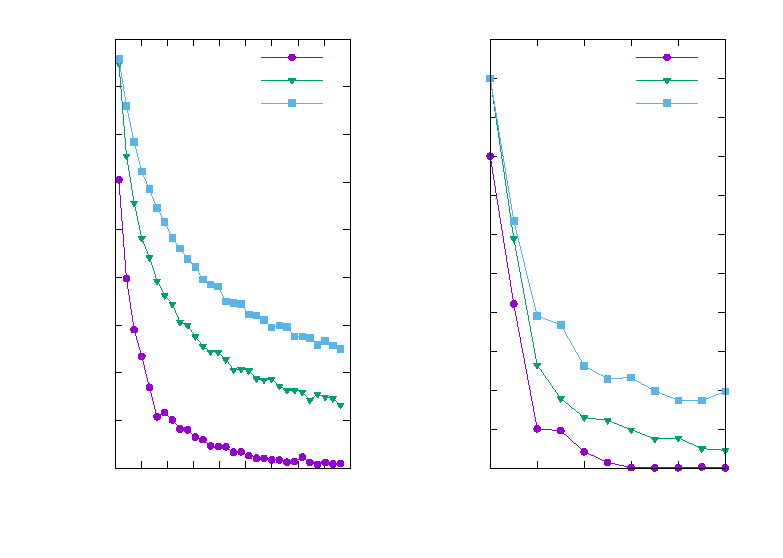
\includegraphics[width={361.00bp},height={253.00bp}]{zigzag-width-strangth}}%
    \gplfronttext
  \end{picture}%
\endgroup
\end{latin}
